% --------------------------------------
% Document Class
% --------------------------------------
\documentclass[a4paper,11pt]{article}
% --------------------------------------



% --------------------------------------
% Use Package
% --------------------------------------


\usepackage[francais]{babel}
%\usepackage{ucs}
\usepackage[utf8]{inputenc}
\usepackage[T1]{fontenc}

\usepackage{makeidx}
\usepackage{color}
\usepackage{graphicx}
\usepackage{float}
\usepackage[hidelinks]{hyperref} 
\usepackage{geometry}
%\usepackage{lastpage}
%\usepackage{marginnote}
\usepackage{fancyhdr}
%\usepackage{titlesec}
%\usepackage{framed}
\usepackage{amsmath}
\usepackage{empheq}
\usepackage{array}
\usepackage{multicol}
\usepackage{csquotes}
%\usepackage{adjustbox}

% insert code
\usepackage{listings}

% define our color
\usepackage{xcolor}

% code color
\definecolor{ligthyellow}{RGB}{250,247,220}
\definecolor{darkblue}{RGB}{5,10,85}
\definecolor{ligthblue}{RGB}{1,147,128}
\definecolor{darkgreen}{RGB}{8,120,51}
\definecolor{darkred}{RGB}{160,0,0}

% other color
\definecolor{ivi}{RGB}{141,107,185}


\lstset{
    language=scilab,
    captionpos=b,
    extendedchars=true,
    frame=lines,
    numbers=left,
    numberstyle=\tiny,
    numbersep=5pt,
    keepspaces=true,
    breaklines=true,
    showspaces=false,
    showstringspaces=false,
    breakatwhitespace=false,
    stepnumber=1,
    showtabs=false,
    tabsize=3,
    basicstyle=\small\ttfamily,
    backgroundcolor=\color{ligthyellow},
    keywordstyle=\color{ligthblue},
    morekeywords={include, printf, uchar},
    identifierstyle=\color{darkblue},
    commentstyle=\color{darkgreen},
    stringstyle=\color{darkred},
}


% --------------------------------------



% --------------------------------------
% Page setting
% --------------------------------------
%\pagestyle{empty}
\setlength{\headheight}{15pt}

\setcounter{secnumdepth}{3}
\setcounter{tocdepth}{2}

\makeatletter
\@addtoreset{chapter}{part}
\makeatother 

\hypersetup{         % parametrage des hyperliens
  colorlinks=true,      % colorise les liens
  breaklinks=true,      % permet les retours à la ligne pour les liens trop longs
  urlcolor= blue,       % couleur des hyperliens
  linkcolor= black,     % couleur des liens internes aux documents (index, figures, tableaux, equations,...)
  citecolor= green      % couleur des liens vers les references bibliographiques
}

% --------------------------------------

% --------------------------------------
% Information
% --------------------------------------
\title{
  \noindent\hrulefill \\
  \vspace{10mm} Compte-rendu TP1 VisA: Callibration de caméra
}

\author{Gaëtan DEFLANDRE}
% --------------------------------------

\definecolor{myColor}{rgb}{0.5, 0.1, 0.75}

% --------------------------------------
% Begin content
% --------------------------------------
\begin{document}


\maketitle

\noindent\hrulefill \\


\section{Introduction}

Dans le domaine de l'optique, nous avons vu que la projection d'un objet 3D sur 
le capteur d'une caméra (plan image à deux dimensions), dépend de plusieurs paramètres:
\begin{itemize}
 \item Les coordonnées homogènes de l'objet dans la scène.
 \item La matrice extrinsèque, qui donne les rotations et translations de la caméra dans scène.
 \item La matrice intrinsèque, qui donne les paramètres internes de la caméra, pouvant changer 
 selon les réglages de la caméra.\\
\end{itemize}

Dans certains cas, les paramètres intrinsèques et/ou extrinsèques de la caméra sont 
inconnus. Il existe plusieurs méthodes pour retrouver ces paramètres.\\

La méthode de Zhang est l'une d'entre elles. Pour appliquer cette méthode, il nous faut 
plusieurs images d'un plan dont les coordonnées sont connues dans la scène. Il faut conserver 
les mêmes réglages pour les différentes images.\\

\newpage

\section{Implémentation sous Scilab}

Pour implémenter la méthode de Zhang, nous utilisons Scilab. La macro se découpe en trois 
parties:
\begin{itemize}
 \item Initialisation des variables.
 \item Approximation de la matrice intrinsèque.
 \item Approximation des matrices extrinsèques.\\
\end{itemize}

$M$ représente les points de la mire dans la scène 3D. $m$ représente les points de la 
projection de la mire sur les plans images 2D, des différentes prises de vues. Nous disposons 
de quatre images, donc quatre 
jeux de valeurs pour $m$. Ces coordonnées sont connues et nous les utiliserons pour les 
calculer. Une lecture de fichier est nécessaire pour initialiser $M$ et $m$.\\


\begin{lstlisting}[caption=Lecture de fichier pour retrouver M et m]
// Nombre d'images
ni = 4;
// Lire les coordonnees des points de la mire dans la scene
M = read('points.txt', -1, 2)';
...
// Boucler pour toutes les images
for i = 1:ni
  // Lire les points de l'image
  m(1:2,:,i) = read('points-'+string(i)+'.txt', -1, 2)';
  m(3,:,i) = ones(1, np);
  ...
end
...
\end{lstlisting}


\subsection{Matrice intrinsèque}

Étant donné que la mire est plane, nous n'avons pas besoin de la profondeur donnée par 
l'axe $Z$, dans les coordonnées de la mire par rapport à la scène. Dans Scilab, cela se 
traduit par: \textbf{M(sansZ,:)}. Nous avons donc: 

\begin{equation}
  \begin{aligned}
    m_i=&A
    \begin{bmatrix}
    r_1 & r_2 & r_3 & t 
    \end{bmatrix}
    \begin{bmatrix}
    X \\ Y \\ 0 \\ 1\\ 
    \end{bmatrix}\\
    m_i=&A
    \begin{bmatrix}
    r_1 & r_2 & t\\
    \end{bmatrix}
    \begin{bmatrix}
    X \\ Y \\ 1
    \end{bmatrix}
  \end{aligned}
\end{equation}

Où $A$ est la matrice intrinsèque caractérisée par:

\begin{equation}
  A=
  \begin{bmatrix}
   \alpha & \gamma & u_0 \\
   0 & \beta & v_0 \\
   0 & 0 & 1 \\
  \end{bmatrix}
\end{equation}

Avec cela, il est possible d'estimer une homographie en considérant les équations 
suivantes (annexe, ligne 24):

\begin{equation}
  \begin{bmatrix}
    h_1 & h_2 & h_3
  \end{bmatrix}
  = \lambda A 
  \begin{bmatrix}
    r_1 & r_2 & t
  \end{bmatrix}
\end{equation}

\begin{equation}
  \begin{aligned}
    h_1^T A^{-T} A^{-1} h_2 &= 0 \\
    h_1^T A^{-T} A^{-1} h_1 &= h_2^T A^{-T} A^{-1} h_2
  \end{aligned}
\end{equation}

Ensuite, nous pouvons retrouver les contraintes d'homographie courante avec 
l'équation suivante (annexe, ligne 26).

\begin{equation}
  v_{ij} = [h_{i1} h_{j1} , h_{i1} h_{j2} + h_{i2} h_{j1} , h_{i2} h_{j2} ,
h_{i3} h_{j1} + h_{i1} h_{j3} , h_{i3} h_{j2} + h_{i2} h_{j3} , h_{i3} h_{j3} ]^T
\end{equation}

Traduit en dans Scilab:

\begin{lstlisting}[caption=Fonction ZhangConstraintTerm]
/// \brief Calcule un terme de contrainte a partir d'une homographie.
///
/// \param H: matrice 3*3 définissant l'homographie.
/// \param i: premiere colonne.
/// \param j: deuxieme colonne.
/// \return vecteur definissant le terme de contrainte.
function v = ZhangConstraintTerm(H, i, j)
  
  // /!\ matrice scilab: M(y,x), soit M(row,col)
  
  // La matrice non transposer
  w = [];
  w(1) = H(1,i) * H(1,j);
  w(2) = (H(1,i) * H(2,j)) + (H(2,i) * H(1,j));
  w(3) = H(2,i) * H(2,j);
  w(4) = (H(3,i) * H(1,j)) + (H(1,i) * H(3,j));
  w(5) = (H(3,i) * H(2,j)) + (H(2,i) * H(3,j));
  w(6) = H(3,i) * H(3,j);
  
  // Transposée de w
  v = w';
endfunction
\end{lstlisting}

Une fois itéré pour chaque image de $m$. Nous pouvons alors en déduire les 
valeurs de $B$, une matrice symétrique, en fonction des différentes estimations 
d'homographies.

\begin{equation}
  B = A^{-T} = A^{-1} =
  \begin{bmatrix}
    B_{11} & B_{12} & B_{11} \\
    B_{12} & B_{22} & B_{23} \\
    B_{13} & B_{23} & B_{33} \\
  \end{bmatrix}
\end{equation}

Les valeurs de $B$ sont calculées et rangées dans un vecteur $b$ (Annexe, ligne 29).\\

Une fois le vecteur $b$ obtenu, nous pouvons approximer les valeurs de la matrice intrinsèque:

\begin{center}
  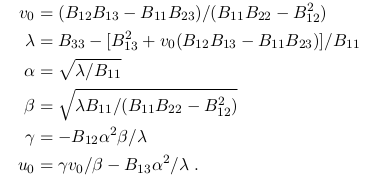
\includegraphics[width=230px]{annexe_b.png}
\end{center}

Voici la fonction dans Scilab:

\begin{lstlisting}[caption=Fonction d'approximation de la matrice intrinsèque à partir de b]
/// \brief Calcule la matrice des parametres intrinseques.
///
/// \param b: vecteur resultant de l'optimisation de Zhang.
/// \return matrice 3*3 des parametres intrinseques.
function A = IntrinsicMatrix(b)
  A = zeros(3, 3);
  
  A(3,3) = 1;
  
  v0 = (b(2)*b(4) - b(1)*b(5)) / (b(1)*b(3) - b(2)*b(2));
  lambda = b(6) - ( (b(4)*b(4) + v0*(b(2)*b(4) - b(1)*b(5))) / b(1) );
  alpha = sqrt(lambda/b(1));
  mybeta = sqrt((lambda*b(1)) / (b(1)*b(3) - b(2)*b(2)))
  mygamma = ((-b(2)) * alpha * alpha * mybeta) / lambda;
  u0 = (mygamma*v0)/mybeta -(b(4)*alpha*alpha)/lambda;
  
  A(1,1) = alpha;
  A(  \begin{bmatrix}
   \alpha & \gamma & u_0 \\
   0 & \beta & v_0 \\
   0 & 0 & 1 \\
  \end{bmatrix}1,2) = mygamma;
  A(1,3) = u0;
  A(2,2) = mybeta;
  A(2,3) = v0;
endfunction
\end{lstlisting}

Nous retrouvons la matrice intrinsèque suivante:

\begin{equation}
  A =
  \begin{bmatrix}
      3498.2767 & - 3.1310503  &  336.76583 \\  
      0.        &   3503.8946  &  220.1142  \\
      0.        &   0.         &  1.\\
  \end{bmatrix}
\end{equation}


\subsection{Matrice extrinsèque}

Maintenant que nous avons estimé les valeurs de $A$, nous pouvons approximation les
matrices extrinsèques pour chaque image de $m$. Nous utilisons les formules suivantes:

\begin{equation}
  \begin{aligned}
    r_1 &= \lambda A^{-1} h_1\\
    r_2 &= \lambda A^{-1} h_2\\
    r_3 &= r_1 * r_2\\
    t &= \lambda A^{-1} h_3\\
  \end{aligned}
\end{equation}

Ce qui nous donne la fonction suivante dans Scilab:

\begin{lstlisting}[caption=Fonction d'approximation de la matrice extrinsèque]
/// \brief Calcule la matrice des parametres extrinseques.
///
/// \param iA: inverse de la matrice intrinseque.
/// \param H: matrice 3*3 definissant l'homographie.
/// \return matrice 3*4 des parametres extrinseques.
function E = ExtrinsicMatrix(iA, H)
  
  lambda = 1 / norm(iA*H(:,1));
  
  r1 = lambda * iA * H(:,1);
  r2 = lambda * iA * H(:,2);
  r3 = r1 .* r2;
  t = lambda * iA * H(:,3);
  
  E = [r1,r2,r3,t];
  disp(E);
endfunction
\end{lstlisting}

Nous retrouvons les matrices extrinsèques suivantes:

\begin{tabular}{|c|c|}
  \hline
  Image 1 
  &
  $\begin{bmatrix}
    0.9999998 &   0.0009052 &   0.0009052 & - 48.811558\\
    0.0000377 &   0.9982948 &   0.0000376 &   54.733305\\
    0.0006696 & - 0.0015763 & - 0.0000011 &   9854.3606
  \end{bmatrix}$
  \\
  \hline
  Image 2 
  & 
  $\begin{bmatrix}
      0.7124496 &   0.0007762 &   0.0005530 & - 46.123202  \\
    - 0.0039703 &   1.0010299 & - 0.0039744 &   43.830318  \\
    - 0.7017120 & - 0.0006379 &   0.0004476 &   7905.8899 
  \end{bmatrix}$
  \\
  \hline
  Image 3 
  & 
  $\begin{bmatrix}
      0.9848432 &   0.1745697 &   0.1719238 & - 43.812292  \\
    - 0.1734468 &   0.9833136 & - 0.1705526 &   49.196563  \\
      0.0002832 &   0.0005524 &   0.0000002 &   8870.6728 
  \end{bmatrix}$
  \\
  \hline
  Image 4
  & 
  $\begin{bmatrix}
      1.        &   0.0045336 &   0.0045336 & - 143.8696   \\
      0.0000023 &   0.7020868 &   0.0000016 &   42.078153  \\
    - 0.0000609 & - 0.714386  &   0.0000435 &   8872.4252 
  \end{bmatrix}$
  \\
  \hline
\end{tabular}

\subsection{Retrouver la focale}

Soit A la matrice intrinsèque de la caméra qui peut s'exprimer par les formules suivantes:

\begin{equation}
  A=
  \begin{bmatrix}
   \alpha & \gamma & u_0 \\
   0 & \beta & v_0 \\
   0 & 0 & 1 \\
  \end{bmatrix}
  =
  \begin{bmatrix}
   k_uf & s_{uv}f & u_0 \\
   0 & k_vf & v_0 \\
   0 & 0 & 1 \\
  \end{bmatrix}
  =
  \begin{bmatrix}
   k_u & s_{uv} & u_0 \\
   0 & k_v & v_0 \\
   0 & 0 & 1 \\
  \end{bmatrix}
  \begin{bmatrix}
    f & 0 & 0 \\
    0 & f & 0 \\
    0 & 0 & 1 \\
  \end{bmatrix}
\end{equation}

Si nous disposons de la taille du capteur en $x$ et en $y$, ainsi que du nombre de 
pixels en $x$ et en $y$ du capteur. Alors, nous retrouver le facteur d'échelle $k_u$ en 
$x$ et $k_v$ en $y$:

\begin{equation}
\begin{aligned}
  k_u &= \frac{nombre\_de\_pixel\_en\_x}{taille\_du\_capteur\_x\_en\_mm} \\
  k_v &= \frac{nombre\_de\_pixel\_en\_y}{taille\_du\_capteur\_y\_en\_mm} 
\end{aligned}
\end{equation}

Donc, nous calculons la focale avec: 

\begin{equation}
\begin{aligned}
  f &= \frac{\alpha}{k_u} \\
  &= \frac{\beta}{k_v}
\end{aligned}
\end{equation}

Si nous disposons des coordonnées du centre de l'image, $u_0$ et $v_0$. Alors,
nous pouvons utiliser ces valeurs exactes plutôt que leurs estimations lors des calculs 
de la matrice intrinsèque dans la méthode Zhang.

\section{Conclusion}

Pour conclure, la méthode Zhang permet de retrouver la matrice intrinsèque et les 
matrices extrinsèques d'images. Ces images doivent convenir un objet plat dont nous 
connaissons les coordonnées dans la scène, ainsi que les coordonnées de l'objet sur 
les différents plans images.\\

Ce type de méthode permet d'appréhender d'autres technologies telles que les tenseurs 
trifocaux.

\section{Annexe}

\begin{lstlisting}[caption=Macro générale qui va appeler les fonctions]
// Definition des fonctions utilitaires
exec ('glue.sci', -1);
exec ('gaetan-deflandre.sci', -1);
// Nombre d'images
ni = 4;

// Lire les coordonnees des points de la mire dans la scene
M = read('points.txt', -1, 2)';
np = size(M, 2);
M = [M; zeros(1, np); ones(1, np)];
sansZ = [1, 2, 4];
// Initialiser la matrice des contraintes
V = [];
// Matrices des homographies
H = zeros(3, 3, ni);
// Coordonnees de tous les points image
m = zeros(3, np, ni);
// Boucler pour toutes les images
for i = 1:ni
  // Lire les points de l'image
  m(1:2,:,i) = read('points-'+string(i)+'.txt', -1, 2)';
  m(3,:,i) = ones(1, np);
  // Estimer l'homographie entre la mire et l' image
  H(:,:,i) = ZhangHomography(M(sansZ,:), m(:,:,i));
  // Ajouter deux lignes de contraintes dans V
  V = [V; ZhangConstraints(H(:,:,i))];
end
// Calculer le vecteur b
b = SmallestRightSingular(V);
// Estimation de la matrice intrinseque
A = IntrinsicMatrix(b);
iA = inv(A);
// Estimations des matrices extrinseques
E = zeros(3, 4, ni);
for i = 1:ni
  E(:,:,i) = ExtrinsicMatrix(iA, H(:,:,i));
end
\end{lstlisting}

\end{document}
